%
% LaTeX report template 
%
\documentclass[a4paper,10pt]{article}
\usepackage{graphicx}
\usepackage{amsmath}
\usepackage{caption}
\usepackage{subcaption}
\usepackage{hyperref}
\usepackage[english]{babel}
\usepackage[latin1]{inputenc}
\usepackage{tikz}
\usepackage{pgfplots}
\pgfplotsset{compat=1.8}
\usepgfplotslibrary{statistics}

\tikzstyle{vertex}=[circle, draw, inner sep=2pt, minimum size=3pt]
\newcommand{\vertex}{\node[vertex]}

\tikzstyle{vecArrow} = [thick, decoration={markings,mark=at position
   1 with {\arrow[semithick]{open triangle 60}}},
   double distance=1.4pt, shorten >= 5.5pt,
   preaction = {decorate},
   postaction = {draw,line width=1.4pt, white,shorten >= 4.5pt}]
\tikzstyle{innerWhite} = [semithick, white,line width=1.4pt, shorten >= 4.5pt]
%
\begin{document}
%
	   \title{Solving the Steiner tree problem by an approximation algorithm }

   \author{E.Bahrami Rad \\ e-mail: s6embahr@uni-bonn.de}
          
   \date{}

   \maketitle
   
   \tableofcontents
 
  \newpage
    
% This is a comment: in LaTeX everything that in a line comes
% after a "%" symbol is treated as comment

% When adding * to \section, \subsection, etc... LaTeX will not assign
% a number to the section

\section{Introduction}
An approximation algorithm for finding a Steiner tree of a connected, undirected distance graph was implemented. This algoritm has approximation ratio of $2-\frac{2}{l}$, which means it gives us a Steiner tree with total distance of all edges at most $2-\frac{2}{l}$ times that of the optimal tree, where $l$ is the number of leaves in the optimal tree. The worst case time complexity of this algorithm is $ \mathcal{O}(\left| V \right|\log{}\left| V \right| + \left| E \right|)$, where E is the set of edges and V is the set of vertices.
 
 
\section{Steiner tree problem}
Given an undirected distance graph $G=(V,E,d)$ and a set S, where E is the set of edges in G, V is the set of vertices in G, d is a distance function which maps E into the set of nonnegative numbers and $S \in V$ is a subset of V. Let Q be any subset of vertices in a connected subgraph G' of G. We shall say that G' spans Q. A spanning tree of G is tree subgraph of G that spans V. The minimal spanning tree of G is a spanning tree of G such that the total distance of on its edges is minimal among all spanning trees. The Steiner tree for a given G and S is the tree that spans S, and the minimal Steiner tree is the one among all Steiner trees for G and S that has minimal total distance.
The problem for finding a minimal Steiner tree for any given G and S has been proved to be NP-Complete[2].	

\begin{figure}[h]
\centering
\begin{subfigure}{0.4\textwidth}
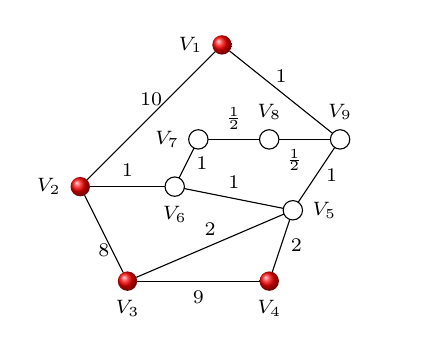
\begin{tikzpicture}[node distance   = 1 cm,scale=0.3]
  %\useasboundingbox (-1,-1) rectangle (11,11); 
  \tikzset{VertexStyle/.style = {circle,
  								  draw,
								  inner sep      = 0pt,
                                 outer sep      = 0pt,
                                 minimum size   = 7 pt}}

  \tikzset{TerminalStyle/.style = {shape 		= circle,
  								  ball color	= red,
  								  text			= black,
								  inner sep		= 0pt,
                                 outer sep		= 0pt,
                                 minimum size	= 7 pt}}
                                 
  \tikzset{EdgeStyle/.style   = {thin}}
                                 
  \tikzset{LabelStyle/.style =   {draw}}
  
     \node[TerminalStyle](V_1) at (6,11) [label=left:\scriptsize $V_1$]{};
     \node[TerminalStyle](V_2) at (0,5) [label=left:\scriptsize $V_2$]{};
	 \node[TerminalStyle](V_3) at (2,1) [label=below:\scriptsize $V_3$]{};
	 \node[TerminalStyle](V_4) at (8,1) [label=below:\scriptsize $V_4$]{};
	 \node[VertexStyle] (V_5) at (9,4) [label=right:\scriptsize $V_5$]{};
	 \node[VertexStyle] (V_6) at (4,5) [label=below:\scriptsize $V_6$]{};
	 \node[VertexStyle] (V_7) at (5,7) [label=left:\scriptsize $V_7$]{};	 
 	 \node[VertexStyle] (V_8) at (8,7) [label=above:\scriptsize $V_8$]{};
 	 \node[VertexStyle](V_9) at (11,7) [label=above:\scriptsize $V_9$]{};    
     \node (imp1) at (11,5) {};
     \node (imp2) at (14,5) {};
        
     \draw[EdgeStyle](V_1) to node[above]{\scriptsize 10} (V_2);
     \draw[EdgeStyle](V_1) to node[above]{\scriptsize 1} (V_9);
     \draw[EdgeStyle](V_2) to node[below]{\scriptsize 8} (V_3);
     \draw[EdgeStyle](V_3) to node[below]{\scriptsize 9} (V_4);
     \draw[EdgeStyle](V_4) to node[right]{\scriptsize 2} (V_5);
     \draw[EdgeStyle](V_3) to node[above]{\scriptsize 2} (V_5);
     \draw[EdgeStyle](V_5) to node[above]{\scriptsize 1} (V_6);
     \draw[EdgeStyle](V_6) to node[above]{\scriptsize 1} (V_2);
     \draw[EdgeStyle](V_6) to node[right]{\scriptsize 1} (V_7);
     \draw[EdgeStyle](V_7) to node[above]{\tiny $\frac{1}{2}$} (V_8);
     \draw[EdgeStyle](V_8) to node[below,pos=0.3]{\tiny $\frac{1}{2}$} (V_9);     
	 \draw[EdgeStyle](V_5) to node[right]{\scriptsize 1} (V_9);    
     %\draw[EdgeStyle](V_2) to node[LabelStyle]{3} (V_1);
 	 
  \end{tikzpicture}
  \caption{Graph G }
  \end{subfigure}
  ~
  \begin{subfigure}{0.4\textwidth}
	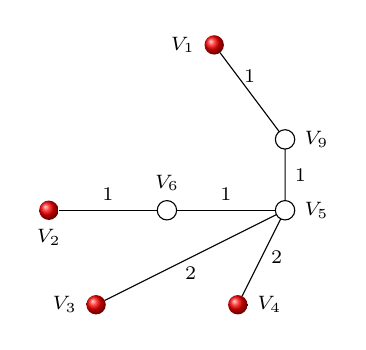
\begin{tikzpicture}[node distance   = 1 cm,scale=0.3]
	  %\useasboundingbox (-1,-1) rectangle (11,11); 
	  \tikzset{VertexStyle/.style = {circle,
	  								  draw,
									  inner sep      = 0pt,
	                                 outer sep      = 0pt,
	                                 minimum size   = 7 pt}}
	
	  \tikzset{TerminalStyle/.style = {shape 		= circle,
	  								  ball color	= red,
	  								  text			= black,
									  inner sep		= 0pt,
	                                 outer sep		= 0pt,
	                                 minimum size	= 7 pt}}
	                                 
	  \tikzset{EdgeStyle/.style   = {thin}}
	                                 
	  \tikzset{LabelStyle/.style =   {draw}}
	  
	     \node[TerminalStyle](V_1) at (7,11) [label=left:\scriptsize $V_1$]{};
	     \node[TerminalStyle](V_2) at (0,4) [label=below:\scriptsize $V_2$]{};
		 \node[TerminalStyle](V_3) at (2,0) [label=left:\scriptsize $V_3$]{};
		 \node[TerminalStyle](V_4) at (8,0) [label=right:\scriptsize $V_4$]{};
		 \node[VertexStyle] (V_5) at (10,4) [label=right:\scriptsize $V_5$]{};
		 \node[VertexStyle] (V_6) at (5,4) [label=above:\scriptsize $V_6$]{};
		 \node[VertexStyle](V_9) at (10,7) [label=right:\scriptsize $V_9$]{};    
	       
	     \draw[EdgeStyle](V_1) to node[above]{\scriptsize 1} (V_9);
	     
	     \draw[EdgeStyle](V_4) to node[right]{\scriptsize 2} (V_5);
	     \draw[EdgeStyle](V_3) to node[below]{\scriptsize 2} (V_5);
	     \draw[EdgeStyle](V_5) to node[above]{\scriptsize 1} (V_6);
	     \draw[EdgeStyle](V_6) to node[above]{\scriptsize 1} (V_2);
	     
		 \draw[EdgeStyle](V_5) to node[right]{\scriptsize 1} (V_9);    
		
		
	  \end{tikzpicture}
	  \caption{Minimal Steiner tree for G}	  
  \end{subfigure}
  \centering
  \caption{Example of Steiner tree problem with terminal set $S=\{V_1,V_2,V_3,V_4 \}$ }
\end{figure}



\section{The approximation algorithm}
\paragraph{}
The algorithm is a modified version of Kou, Markowsky and Berman[3], which gives a better running time and also because of reducing the problem to shortest path and minimum spanning tree it is simpler.
Given $G=(V,E,d)$ a connceted, undirected distance graph, and the set of terminals $S \subseteq V$. Then the graph $G'_1 = (S, E'_1,d'_1)$ can be cosntructed as follows.

For every vertex $s \in S$ let N(s) be the set of vertices in V which are closer to s than to any other vertex in S(in computational geometry N(s) is called the Voronoi region of vertex s). We can partition V according to N(s) by considering $ \{ N(s); s \in S  \} $, in other words every vertex $ v\in V $ belongs uniquely to one of the partitions N(s) with s as its center, where v is closer to s than any other vertex $ q\in S$ , $q \neq s$. Now, the graph $G'_1 = (S, E'_1,d'_1)$ is defined by



\begin{flushleft} 
\begin{equation}\label{EP1}
\begin{split}
 E'_1 = \{(s,t); s,t\in S \  and\ there\ is\ an\ edge\\  (u,v)\in E \ with \ u\in N(s), v \in N(t) \}
\end{split}
\end{equation}
\end{flushleft}
and

\begin{flushleft}
\begin{equation}\label{dp1}
\begin{split}
d'_1(s,t) = min \{d_1(s,u)+d(u,v)+d_1(v,t);\\ (u,v)\in E , u\in N(s), v\in N(t) \}.
\end{split}
\end{equation}

In equation \ref{dp1} $ d_1(v_i,v_j)$ is equal to the distance of shortest path from $v_i$ to $v_j$ for $v_i,v_j \in V$ in graph G.
   
\end{flushleft}
$d'_1(s,t)$ in equation \ref{dp1} is the length of shortest path in G restricted to $N(s) \bigcup N(t)$. And the edge $(u',v')\in E'_1$ corresponds to the bridge edge $(u,v) \in E$ which acts like a bridge that goes from region N(s) to region N(t). Now the algorithm is as follow :\\
	{\em 
	\begin{enumerate}
			\item Construct the graph $G'_1=(S,E'_1,d'_1)$ 
			
			\item Find a minimum spanning tree $G_2$ of $G'_1$.
					
			\item Construct a subgraph $G_3$ of G by replacing each edge in $G_2$ by its corresponding shortest path in G.
					
			\item Find a minimum spanning tree $G_4$ of $G_3$.		
			\item Construct a Steiner tree $G_5$ from $G_4$ by deleting edges in $G_4$, if necessary, so that no leaves in $G_5$ from the set $V-S$ 
		\end{enumerate}	
	\begin{center}
	Algorithm 1
	\end{center}
	}
Step 1 of Algorithm 1 dominates the computational time. This step requires the solution of a single shortest path problem which takes $ \mathcal{O}(|V|\log{} |V| + |E|)$ by using Dijkstra algorithm and Fibonacci heaps[4].

\section{Implementation}
\paragraph{}
Step 1 of Algorithm 1 requires the voronoi region $\{ N(s); s\in S \}$ of each vertex $v\in V$. The partition $\{ N(s); s\in S \}$ can be computed by adjoining an auxiliary vertex $ S_0 $ and edges $ (s_0,s ),s \in S $, with length 0 to G and then performing a single source shortest path with source $s_0$. This step was implemented in the program by using a min priority queue based on a priority heap.The priority queue provides $ \mathcal{O}(log(n)) $ time for enqueing and dequeing. For the Dijkstra algorithm the priority queue stores at most $|V|$ number of item, thus each of enqueing and dequeing need $ \mathcal{O}(log(|V|)) $ and totally there are $|E|$ number of such operations, which gives the running time of $ \mathcal{O}(\left| E \right|\log{} |V|)$ for step 1. This step also needs $\mathcal{O}(|E|)$ for finding $G'_1$ edges. For finding $G'_1$'s edges the program goes through all edges $(u,v)\in E$ and generates the triples $(s(u),s(v),d_1(s(u),u)+d(u,v)+d_1(v,s(v))$ in which $s(v)\in S$ is the center of region that v belongs to.Then the program finds the minimum distance for edge $(s(u),s(v)$ over all distances $d_1(s(u),u)+d(u,v)+d_1(v,s(v))$.   
\paragraph{}
Step 2 computes the minimum spanning tree $G_2$ of $G'_1$. The graph $G'_1$ has $\mathcal{O} (|E|)$ edges and hence this step can be carried out in $\mathcal{O}(|E|log(|S|))$ by using Kruskal algorithm and Union Find data structure[4].
\paragraph{}
In step 3 the edges of $G_2$ have to be replaced by its corresponding edges from the shortest path computed in step 1.Consider the edge $(u,v)$ of $G_2$, this edge corresponds to the shortest path between u and v in the graph G, here all the edges of G from this shortest path are plugged back to $G_2$. In step 1 the predecessor of each vertex has been computed and stored in an array, hence by means of this array the shortest path can be constructed.\\
Step 4 is the same is step 2 in which the minimum spanning tree of the graph from step 3 was computed. A


\section{Results}
Several tests has been performed to evaluate the performance of this aproximation algorithm. The code is implemented in Java 1.8 and the dataset from 11th DIMACS Implementation Challenge[5] is used. All runs are performed on a machine with score 181.433863(the score is calculated according to DIMACS Implementaion Challenge benchmark code to compare the results from different machines).  

\begin{figure}[h]
\centering
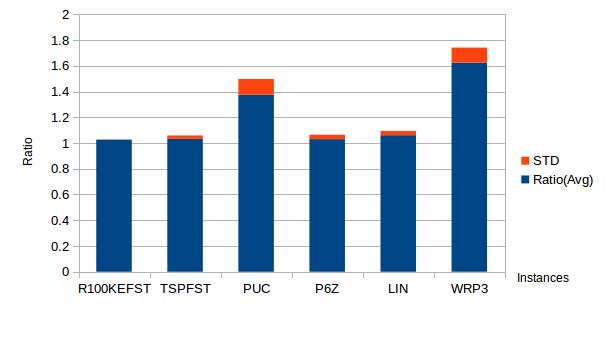
\includegraphics[scale=0.4]{ratio.jpg}
\caption{Comparing approximation ratio over instances of Steiner tree problem}
\end{figure}
The ratio in Figure 2 is the average(arithmetic mean) of several instances for each kind.
R100KEFST, is the instance with fractional weight, Euclidean distance. TSPFST, PUC, P6Z and LIN are the instances of \emph{SteinLib}[6] testsets.

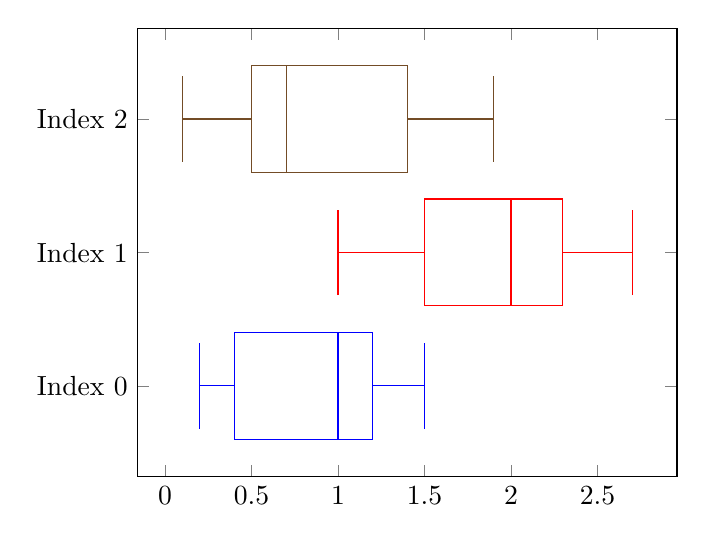
\begin{tikzpicture}
  \begin{axis}
    [
    ytick={1,2,3},
    yticklabels={Index 0, Index 1, Index 2},
    ]
    \addplot+[
    boxplot prepared={
      median=1,
      upper quartile=1.2,
      lower quartile=0.4,
      upper whisker=1.5,
      lower whisker=0.2
    },
    ] coordinates {};
    \addplot+[
    boxplot prepared={
      median=2,
      upper quartile=2.3,
      lower quartile=1.5,
      upper whisker=2.7,
      lower whisker=1
    },
    ] coordinates {};
    \addplot+[
    boxplot prepared={
      median=0.7,
      upper quartile=1.4,
      lower quartile=0.5,
      upper whisker=1.9,
      lower whisker=0.1
    },
    ] coordinates {};
  \end{axis}
\end{tikzpicture}
  

\section{Conclusions}
We have presented an implementation of an approximation algorithm for Steiner tree problem. The algorithm has approximation ratio of $2 - \frac{2}{l}$,where $ l $ is the minimum number of leaves in any Steiner tree for the given graph. The algorithm running time is dominated by a single shortest path problem which is computed in our code using Dijkstra algorithm and priority queue which yields the running time of $\mathcal{O}(|E|log|V|)$.   


% TABLES



\begin{thebibliography}{}

  \bibitem{mehl} Mehlhorn, K. 1987,
      A faster approximation algorithm for the Steiner problem in graphs,
      Information Processing Letters 27, 125-128

  \bibitem{karp72} Karp, R.M. 1972,
      \newblock Reducibility among combinatorial problems,
      \newblock {\em In R. E. Miller and J. W. Thatcher (editors). Complexity of Computer Computations.} New York: Plenum. pp. 85-103.
	
	 \bibitem{kmb} L. Kou, G. Markowsky, and L. Berman
	     \newblock A Fast Algorithm for Steiner Trees
	     \newblock {\em Acta Informatica}, 15,141-145(1981)   
	
	
	\bibitem{FIBH}  M.L. Fredman and R.E. Tarjan, Fibonacci Heaps 
	and Their Uses in Improved Network Optimization Algorithms(IEEE, 1984) 338-246

	\bibitem{shp}  Sariel Har-Peled,
	\newblock Greedy Algorithms for Minimum
	Spanning Trees, CS 473: Fundamental Algorithms, Fall 2011,
	\url{https://courses.engr.illinois.edu/cs473/fa2011/lec/12_notes.pdf}
	
	\bibitem{DIMACS} 11th DIMACS Implementation Challenge in Collaboration with ICERM:
		Steiner Tree Problems,
		\url{http://dimacs11.zib.de/downloads.html}	
	
	\bibitem{SteinLib} SteinLib Testdata Library,
		SteinLib is a collection of Steiner tree problems in graphs and variants.
			\url{http://steinlib.zib.de/steinlib.php}
	
	
\end{thebibliography}

\end{document}

